\documentclass{article}

\usepackage{fancyhdr}
\usepackage{extramarks}
\usepackage{amsmath}
\usepackage{amsthm}
\usepackage{amsfonts}
\usepackage{tikz}
\usepackage{multicol}
\usepackage{float}
%\usepackage[plain]{algorithm}
\usepackage[ruled,vlined]{algorithm2e}
\usepackage{algpseudocode}

\usetikzlibrary{automata,positioning}

%
% Basic Document Settings
%

\topmargin=-0.45in
\evensidemargin=0in
\oddsidemargin=0in
\textwidth=6.5in
\textheight=9.0in
\headsep=0.25in

\linespread{1.1}

\pagestyle{fancy}
\lhead{\hmwkAuthorName}
\chead{\hmwkClass\ : \hmwkTitle}
\rhead{\firstxmark}
\lfoot{\lastxmark}
\cfoot{\thepage}

\renewcommand\headrulewidth{0.4pt}
\renewcommand\footrulewidth{0.4pt}

\setlength\parindent{0pt}

%
% Create Problem Sections
%

\newcommand{\enterProblemHeader}[1]{
    \nobreak\extramarks{}{Problem \arabic{#1} continued on next page\ldots}\nobreak{}
    \nobreak\extramarks{Problem \arabic{#1} (continued)}{Problem \arabic{#1} continued on next page\ldots}\nobreak{}
}

\newcommand{\exitProblemHeader}[1]{
    \nobreak\extramarks{Problem \arabic{#1} (continued)}{Problem \arabic{#1} continued on next page\ldots}\nobreak{}
    \stepcounter{#1}
    \nobreak\extramarks{Problem \arabic{#1}}{}\nobreak{}
}

\setcounter{secnumdepth}{0}
\newcounter{partCounter}
\newcounter{homeworkProblemCounter}
\setcounter{homeworkProblemCounter}{1}
\nobreak\extramarks{Problem \arabic{homeworkProblemCounter}}{}\nobreak{}

%
% Homework Problem Environment
%
% This environment takes an optional argument. When given, it will adjust the
% problem counter. This is useful for when the problems given for your
% assignment aren't sequential. See the last 3 problems of this template for an
% example.
%
\newenvironment{homeworkProblem}[1][-1]{
    \ifnum#1>0
        \setcounter{homeworkProblemCounter}{#1}
    \fi
    \section{Problem \arabic{homeworkProblemCounter}}
    \setcounter{partCounter}{1}
    \enterProblemHeader{homeworkProblemCounter}
}{
    \exitProblemHeader{homeworkProblemCounter}
}

%
% Homework Details
%   - Title
%   - Due date
%   - Class
%   - Section/Time
%   - Instructor
%   - Author
%

\newcommand{\hmwkTitle}{Homework\ \#2}
\newcommand{\hmwkDueDate}{Nov. 6, 2019}
\newcommand{\hmwkClass}{Modern Computational Statistics}
\newcommand{\hmwkClassTime}{ }
\newcommand{\hmwkClassInstructor}{}
\newcommand{\hmwkAuthorName}{\textbf{Huang Daoji}}

%
% Title Page
%

\title{
    \vspace{2in}
    \textmd{\textbf{\hmwkClass:\ \hmwkTitle}}\\
    \normalsize\vspace{0.1in}\small{Due\ on\ \hmwkDueDate\ at 3:10pm}\\
    \vspace{0.1in}\large{\textit{\hmwkClassInstructor\ \hmwkClassTime}}
    \vspace{3in}
}

\author{\hmwkAuthorName}
\date{}

\renewcommand{\part}[1]{\textbf{\large Part \Alph{partCounter}}\stepcounter{partCounter}\\}

%
% Various Helper Commands
%

% Useful for algorithms
\newcommand{\alg}[1]{\textsc{\bfseries \footnotesize #1}}

% For derivatives
\newcommand{\deriv}[1]{\frac{\mathrm{d}}{\mathrm{d}x} (#1)}

% For partial derivatives
\newcommand{\pderiv}[2]{\frac{\partial}{\partial #1} (#2)}

% Integral dx
\newcommand{\dx}{\mathrm{d}x}

% Alias for the Solution section header
\newcommand{\solution}{\textbf{\large Solution}}

% Probability commands: Expectation, Variance, Covariance, Bias
\newcommand{\E}{\mathrm{E}}
\newcommand{\Var}{\mathrm{Var}}
\newcommand{\Cov}{\mathrm{Cov}}
\newcommand{\Bias}{\mathrm{Bias}}

\begin{document}

%\maketitle

\pagebreak

\begin{homeworkProblem}
    \textbf{(1)} \\
    By integrating the pdf, we have the CDF of standard Laplace distribution is
    \begin{equation*}
        F(x) = \left\{
                    \begin{aligned}
                        \frac{1}{2}e^{x} & \quad x < 0 \\
                        1 - \frac{1}{2}e^{-x} & \quad x \geq 0 \\
                    \end{aligned}
               \right.
    \end{equation*}
    So, to generate a standard Laplace random variable, first generate $x \sim U(0, 1)$, then by solving $F(y) = x$, we have $y$ being a sample from standard Laplace distribution. The correctness of this algorithm is shown in class by verifying $P(a \leq y \leq b) = F(b) - F(a)$. \\
        \begin{algorithm}[H]
            \SetAlgoLined
            \caption{get\_laplace\_sample}
            \KwResult{sample from standard Laplace distribution}
            \Begin{
                generate $x \sim U(0, 1)$ \\
                \eIf{$x \geq \frac{1}{2}$}{
                    $res = -\log(2 - 2x)$
                }{
                    $res = \log(2x)$
                }
                \KwRet{res}
            }
        \end{algorithm}
    Below is a histograph of sampling results with groundtruth function. \\
        \begin{figure}[H]
            \centering
            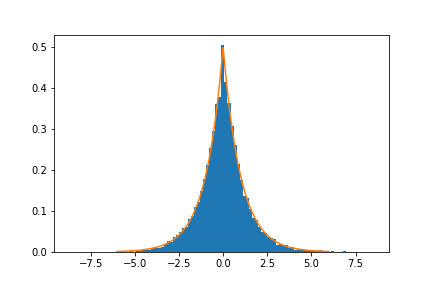
\includegraphics[width=0.5\textwidth]{Laplace.png}
            \caption{histograph of samples generated}
            \label{1}
        \end{figure}
    \textbf{(2)} \\
    To guarantee $k$ times Laplace density can serve as a envelop function for standard Gaussian $N(0, 1)$, we solve
    \begin{equation*}
        \begin{aligned}
            \frac{1}{2}k e^{-|x|} &\geq \frac{1}{\sqrt{2 \pi}} e^{-\frac{x^2}{2}}, \quad \forall x \\
            k & \geq \sqrt{\frac{2e}{\pi}} \\
        \end{aligned}
    \end{equation*}
    So the rejection sampling algorithm is shown below with $k = \sqrt{\frac{2e}{\pi}}$. \\
    \begin{algorithm}[H]
        \SetAlgoLined
        \caption{sample\_normal\_from\_laplace}
        \Begin{
            laplace sample $x_{L}$ = get\_laplace\_sample() \\
            accept probability $p_{acc} = e^{-\frac{1}{2}(|x| - 1)^{2}}$ \\
            decision $accept = Binomial(p_{acc})$ \\
            \eIf{$accept == 1$}{
                \KwRet{$x_{L}$}
            }{
                run again
            }
        }
    \end{algorithm}
    And sampling result is shown below.
    \begin{figure}[H]
        \centering
        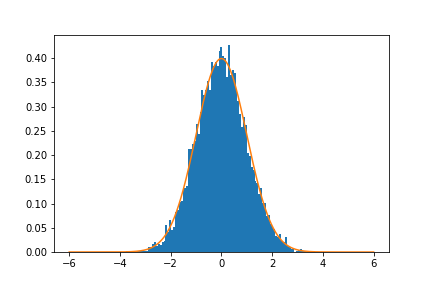
\includegraphics[width=0.5\textwidth]{Gaussian.png}
        \caption{histograph of samples generated}
        \label{2}
    \end{figure}

    \textbf{(3)} \\
    No. Similar to the choice of $k$ in \textbf{(2)}, we have
    \begin{equation*}
        \frac{1}{2}e^{-|x|} \leq \frac{k}{\sqrt{2 \pi}} e^{-\frac{x^2}{2}}, \quad \forall x
    \end{equation*}
    No $k \in R$ satisfy the above equation as $x \to \infty$, so we cannot simulate Laplace RV using $N(0, 1)$ as envelop function.

\end{homeworkProblem}

\begin{homeworkProblem}
    \textbf{(1)} \\
    First, we have the probability of $(\mu, \sigma)$ given the observed data (up to a normalsizing constant)
    \begin{equation*}
        \begin{aligned}
            p(\mu, \sigma^2 | X) &\propto p(\mu)p(\sigma^2)p(X | \mu, \sigma^2) \\
            &\propto e^{-\frac{(\mu - \mu_0)^2}{2\tau_0^2}} \frac{e^{-\frac{\nu_0 \sigma_0^2}{2\sigma^2}}}{\sigma^{2 + \nu_0}} \prod \frac{1}{\sigma} e^{-\frac{(x_i - \mu)^2}{2\sigma^2}}\\
        \end{aligned}
    \end{equation*}
    To derive the conditional probability $p(\mu | \sigma^2, X)$, we can a) simply ignore all terms only related to $\sigma$, since they will be integrated out and hence constant, and b) for all terms related to $\mu$, treat the $\sigma$ as a fixed constant. We then have
    \begin{equation*}
        \begin{aligned}
            p(\mu | \sigma^2, X) &\propto exp(-\frac{(\mu - \mu_0)^2}{2\tau_0^2}- \sum \frac{(x_i - \mu)^2}{2\sigma^2}) \\
            &\propto exp(-(\frac{1}{2\tau_0^2} + \frac{n}{2\sigma_2})\mu^2 + (\frac{\mu_0}{\tau_0^2} + \frac{\sum x_i}{\sigma^2})\mu) \\
            &\propto exp(-\frac{(\mu - \frac{\frac{\mu_0}{\tau_0^2} + \frac{\sum x_i}{\sigma^2}}{\frac{1}{\tau_0^2} + \frac{n}{\sigma_2}})^2}{2\frac{1}{\frac{1}{\tau_0^2} + \frac{n}{\sigma_2}}}).
        \end{aligned}
    \end{equation*}
    This implies $\mu \sim N( \frac{\frac{\mu_0}{\tau_0^2} + \frac{\sum x_i}{\sigma^2}}{\frac{1}{\tau_0^2} + \frac{n}{\sigma_2}},  \frac{1}{\frac{1}{\tau_0^2} + \frac{n}{\sigma_2}})$.
    Similarly,
    \begin{equation*}
        \begin{aligned}
            p(\sigma^2 | \mu, X) &\propto \frac{1}{\sigma^{2 + \nu_0 + n}} e^{-\frac{\nu_0\sigma_0^2 + \sum (x_i - \mu)^2}{2\sigma^2}}, \\
        \end{aligned}
    \end{equation*}
    which means $\sigma^2 \sim \text{Inv-}\chi^2(\nu_0 + n, \frac{\nu_0\sigma_0^2 + \sum (x_i - \mu)^2}{\nu_0 + n})$.
    \\ \\
    \textbf{(2)} \\
    \begin{algorithm}[H]
        \SetAlgoLined
        \caption{gibbs\_sampler}
        \KwResult{sample from gibbs sampling}
        \Begin{
            generate $\mu \sim N(0, 1)$ \\
            generate $\sigma^2 \sim \text{Inv-}\chi^2(1, 1)$ \\
            \While{$\#\ of\ samples \leq 1000$}{
                $\mu \sim p(\mu | \sigma^2, X)$ \\
                $\sigma^2 \sim p(\sigma^2 | \mu, X)$ \\
            }
        }
    \end{algorithm}
    Trace plot of $\mu, \sigma$ is shown below.(Note: not $\sigma^2$)
    \begin{figure}[H]
        \centering
        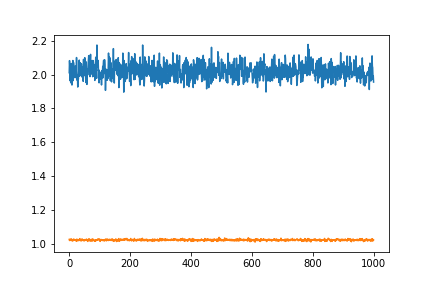
\includegraphics[width=0.5\textwidth]{gibbs.png}
        \caption{trace plot of samples generated}
        \label{3}
    \end{figure}

    \textbf{(3)} \\
    \begin{algorithm}[H]
        \SetAlgoLined
        \caption{metropolis\_sampler}
        \KwResult{sample from metropolis sampling}
        \Begin{
            generate $\mu \sim N(0, 1)$ \\
            generate $\sigma^2 \sim \text{Inv-}\chi^2(1, 1)$ \\
            \While{$\#\ of\ samples \leq 1000$}{
                $\mu' \sim N(\mu | step\_mu)$ \\
                $\sigma'^2 \sim exp(U(-step\_sigma, step\_sigma)) \sigma^2 $ \\
                accept the new $\mu', \sigma'$ with probability $\min(1, exp(\text{log\_likelihood}(\mu', \sigma'^2) - \text{log\_likelihood}(\mu, \sigma^2)))$ \\
            }
        }
    \end{algorithm}
    Trace plot of $\mu, \sigma$ is shown below with step\_mu and step\_sigma being 0.04.(Note: not $\sigma^2$)
    \begin{figure}[H]
        \centering
        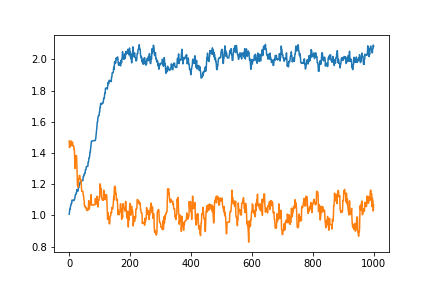
\includegraphics[width=0.5\textwidth]{metropolis.png}
        \caption{trace plot of samples generated}
        \label{3}
    \end{figure}

    \textbf{(4)} \\
    Trace plots and ACF plots are shown below, with $i \geq 200$ being burn-in phase, the first 200 sample are therefore discarded for ACF.
    \begin{figure}[H]
        \centering
        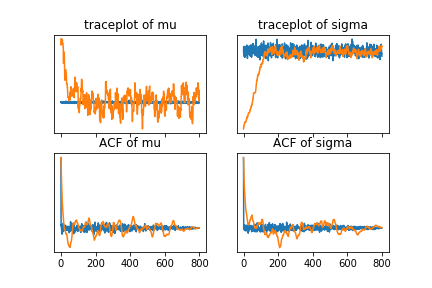
\includegraphics[width=0.5\textwidth]{analysis.png}
        \caption{trace plot of samples generated, above: 1k samples, below: 800}
        \label{4}
    \end{figure}
    Gibbs sampler is better in this case, which has more stable and less correlated samples, and burns in fast. That is because Gibbs sampler makes use of the conditional distribution in this problem.
\end{homeworkProblem}

\begin{homeworkProblem}

    \textbf{(1)} \\
    The scatter plot of HMC samples are shown below. \\
    \begin{figure}[H]
        \centering
        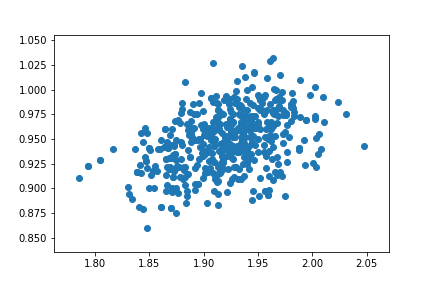
\includegraphics[width=0.5\textwidth]{hmc_res.png}
        \caption{scatter plot of samples generated by HMC}
        \label{4}
    \end{figure}
    Below are figures of ACFs of samples by a) HMC with fixed L, b) HMC with random L, as L increase from 10 to 90. The left 3 * 3 grid are results from HMC with fixed L, while the right 3 * 3 from HMC with random L. We see samples are more stable and robust to change of L when L are sampled. That is because when L are sampled, HMC are able to choose a diverse L, which will 1) enable HMC to sample from local points \textbf{and} 2) enable HMC to tarvel far away out of possible local maxima, whereas a fixed L will force HMC to either 1) travel far away \textbf{or} 2) stay in local modes.\\
    \begin{figure}[H]
        \centering
        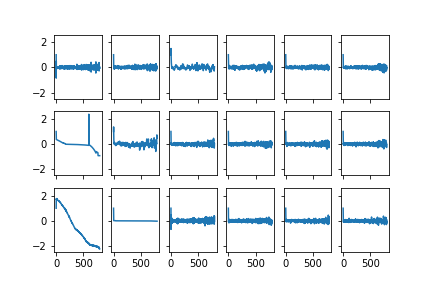
\includegraphics[width=0.5\textwidth]{HMC_step.png}
        \caption{ACF of fixed L(left), and random L(right)}
        \label{4}
    \end{figure}

    \textbf{(2)} \\
    We evaluate each algorithm by applying a sliding window of 1k samples from each algorithm and calculate the KL divergence to GT 1k samples from HMC(down sampled from 50k samples). The above plot are smoothed by a Gaussian filter(with sigma 4). As for implementation and hyperparameters, we applied lr decay for SGLD, and not for SGHMC and SGNHT. SGHMC and SGNHT are runned with $\epsilon = 0.001, C = 10$, which yields best results in SGNHT's original paper and turns out to be the best in my experiments. We show the results of different SGHMC methods in terms of KL divergence to GT(by a long HMC) below. \\

    \begin{figure}[!htb]
    \minipage{0.49\textwidth}
      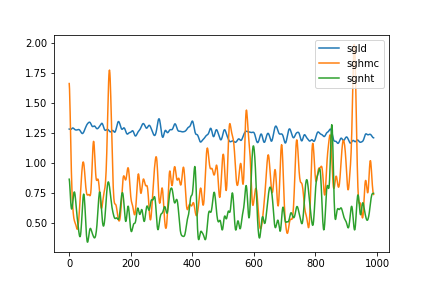
\includegraphics[width=\linewidth]{SGHMC.png}
      \caption{KL with batch\_size=32}\label{fig:awesome_image1}
    \endminipage\hfill
    \minipage{0.49\textwidth}%
      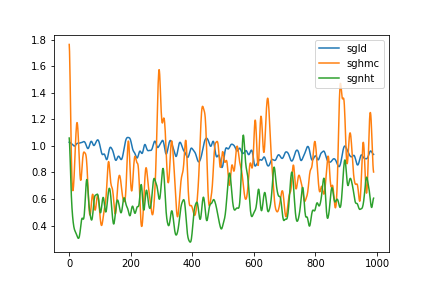
\includegraphics[width=\linewidth]{SGHMC_64.png}
      \caption{KL with batch\_size=64}\label{fig:awesome_image3}
    \endminipage
    \end{figure}

    \begin{figure}[!htb]
    \minipage{0.49\textwidth}
      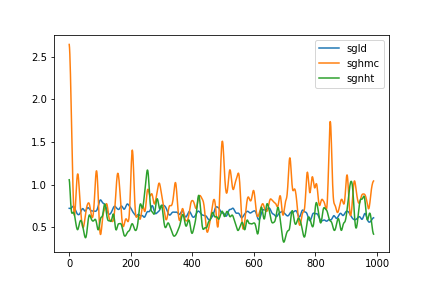
\includegraphics[width=\linewidth]{SGHMC_128.png}
      \caption{KL with batch\_size=128}\label{fig:awesome_image1}
    \endminipage\hfill
    \minipage{0.49\textwidth}%
      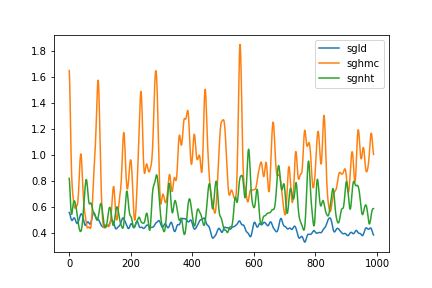
\includegraphics[width=\linewidth]{SGHMC_256.png}
      \caption{KL with batch\_size=256}\label{fig:awesome_image3}
    \endminipage
    \end{figure}

    We can conclude that
    \begin{itemize}
        \item as for performance, SGLD $<$ SGHMC $<$ SGNHT
        \item for convergence rate and average KL after convergence, SGLD $<$ SGHMC $<$ SGNHT(refer to the plot below for more consistant comparation with lr being the same for all methods)
        \item SGLD seems to be stuck somewhere, while SGHMC and SGNHT are generally better(I chose a small learning rate for SGHMC and SGNHT so the var. seems quite high)
        \item SGLD is more sensitive to batch size and learning rate, we also show a plot of three algorithms with the same bs and lr.
    \end{itemize}

    \begin{figure}[H]
        \centering
        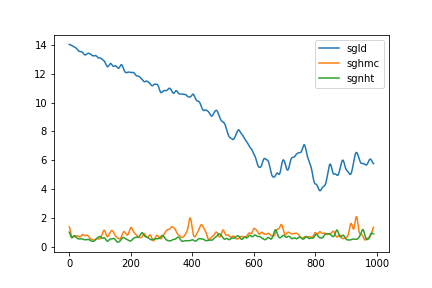
\includegraphics[width=0.5\textwidth]{SGHMC_256_fixlr.png}
        \caption{KL of different SGHMC methods with the same lr}
        \label{4}
    \end{figure}

\end{homeworkProblem}


\end{document}
